\documentclass[11pt]{article}
\usepackage{amssymb, amsthm, amsmath}
\usepackage{bm}
\usepackage{graphicx}
\usepackage[authoryear]{natbib}
\usepackage{bm}
\usepackage{verbatim}
\usepackage{lineno}
\usepackage{times}
\usepackage{soul}
\usepackage{color}
\usepackage{enumitem}
\usepackage{setspace}
\usepackage{times}
\usepackage{changepage}

\usepackage[left=1in,top=1in,right=1in]{geometry}
\pdfpageheight 11in
\pdfpagewidth 8.5in
\linespread{2.0}
\newcommand{\btheta}{ \mbox{\boldmath $\theta$}}
\newcommand{\bmu}{ \mbox{\boldmath $\mu$}}
\newcommand{\balpha}{ \mbox{\boldmath $\alpha$}}
\newcommand{\bbeta}{ \mbox{\boldmath $\beta$}}
\newcommand{\bdelta}{ \mbox{\boldmath $\delta$}}
\newcommand{\blambda}{ \mbox{\boldmath $\lambda$}}
\newcommand{\bgamma}{ \mbox{\boldmath $\gamma$}}
\newcommand{\brho}{ \mbox{\boldmath $\rho$}}
\newcommand{\bpsi}{ \mbox{\boldmath $\psi$}}
\newcommand{\bepsilon}{ \mbox{\boldmath $\epsilon$}}
\newcommand{\bomega}{ \mbox{\boldmath $\omega$}}
\newcommand{\bOmega}{ \mbox{\boldmath $\Omega$}}
\newcommand{\bDelta}{ \mbox{\boldmath $\Delta$}}
\newcommand{\bSigma}{ \mbox{\boldmath $\Sigma$}}
\newcommand{\bPsi}{\mbox{\boldmath $\Psi$}}
\newcommand{\bOne}{\mbox{\boldmath $1$}}
\newcommand{\omu}{\overline{\mu}}
\newcommand{\oSigma}{\overline{\Sigma}}
\newcommand{\Yt}{{\tilde Y}}
\newcommand{\bA}{ \mbox{\bf A}}
\newcommand{\bP}{ \mbox{\bf P}}
\newcommand{\bx}{ \mbox{\bf x}}
\newcommand{\bX}{ \mbox{\bf X}}
\newcommand{\bB}{ \mbox{\bf B}}
\newcommand{\bZ}{ \mbox{\bf Z}}
\newcommand{\by}{ \mbox{\bf y}}
\newcommand{\bY}{ \mbox{\bf Y}}
\newcommand{\bz}{ \mbox{\bf z}}
\newcommand{\bh}{ \mbox{\bf h}}
\renewcommand{\bm}{ \mbox{\bf m}}
\newcommand{\br}{ \mbox{\bf r}}
\newcommand{\bt}{ \mbox{\bf t}}
\newcommand{\bs}{ \mbox{\bf s}}
\newcommand{\bb}{ \mbox{\bf b}}
\newcommand{\bL}{ \mbox{\bf L}}
\newcommand{\bu}{ \mbox{\bf u}}
\newcommand{\bv}{ \mbox{\bf v}}
\newcommand{\bV}{ \mbox{\bf V}}
\newcommand{\bW}{ \mbox{\bf W}}
\newcommand{\bG}{ \mbox{\bf G}}
\newcommand{\bH}{ \mbox{\bf H}}
\newcommand{\bw}{ \mbox{\bf w}}
\newcommand{\bo}{ \mbox{\bf o}}
\newcommand{\bfe}{ \mbox{\bf e}}
\newcommand{\iid}{\stackrel{iid}{\sim}}
\newcommand{\ind}{\stackrel{ind}{\sim}}
\newcommand{\dd}{\; \text{d} }
\newcommand{\ddd}{\text{d} }
\newcommand{\indep}{\stackrel{indep}{\sim}}
\newcommand{\converged}{\stackrel{d}{\rightarrow}}
\newcommand{\calR}{{\cal R}}
\newcommand{\calG}{{\cal G}}
\newcommand{\calD}{{\cal D}}
\newcommand{\calS}{{\cal S}}
\newcommand{\calB}{{\cal B}}
\newcommand{\calA}{{\cal A}}
\newcommand{\calT}{{\cal T}}
\newcommand{\calO}{{\cal O}}
\newcommand{\argmax}{{\mathop{\rm arg\, max}}}
\newcommand{\argmin}{{\mathop{\rm arg\, min}}}
\newcommand{\Frechet}{\mbox{Fr$\acute{\mbox{e}}$chet }}
\newcommand{\Matern}{\mbox{Mat$\acute{\mbox{e}}$rn }}
\newcommand{\ballunion}{B_a(\bs_1) \cup B_b(\bs_2) }

\newcommand{\beq}{ \begin{equation}}
\newcommand{\eeq}{ \end{equation}}
\newcommand{\beqn}{ \begin{eqnarray}}
\newcommand{\eeqn}{ \end{eqnarray}}

\newcommand*\patchAmsMathEnvironmentForLineno[1]{%
  \expandafter\let\csname old#1\expandafter\endcsname\csname #1\endcsname
  \expandafter\let\csname oldend#1\expandafter\endcsname\csname end#1\endcsname
  \renewenvironment{#1}%
     {\linenomath\csname old#1\endcsname}%
     {\csname oldend#1\endcsname\endlinenomath}}%
\newcommand*\patchBothAmsMathEnvironmentsForLineno[1]{%
  \patchAmsMathEnvironmentForLineno{#1}%
  \patchAmsMathEnvironmentForLineno{#1*}}%
\AtBeginDocument{%
\patchBothAmsMathEnvironmentsForLineno{equation}%
\patchBothAmsMathEnvironmentsForLineno{align}%
\patchBothAmsMathEnvironmentsForLineno{flalign}%
\patchBothAmsMathEnvironmentsForLineno{alignat}%
\patchBothAmsMathEnvironmentsForLineno{gather}%
\patchBothAmsMathEnvironmentsForLineno{multline}%
}



\begin{document}\linenumbers

\begin{center}
{\Large {\bf A spatial model for rare binary events}}\\
\today
\end{center}

\section{Introduction}\label{rbs:intro}

The goal in binary regression is to relate a latent variable to a response using a link function.
% $g$ so that P$(Y_i=1) = \pi_i= g(\bX_i \bbeta)$, where $\bX_i$ is the vector of covariates for observation $i$, and $\bbeta$ is the $p$-vector of regression coefficients.
Two common examples of binary regression include logistic regression
% with $\pi_i = \frac{ \exp{\bX_i \bbeta} }{1 + \exp{\bX_i \bbeta}}$
and probit regression.
% with $\pi_i = \Phi(\bX_i \bbeta)$ where $\Phi(\cdot)$ represents the standard normal distribution function.
The link functions for logistic and probit regression are symmetric, so they may not be well-suited for asymmetric data.
% In the case that $\xi = 0$, this is the complementary log-log (cloglog) link function.
An asymmetric alternative to these link functions is the complementary log-log (cloglog) link function.
More recently, \citet{Wang2010} introduced the generalized extreme value (GEV) link function for rare binary data.
The GEV link function introduces a new shape parameter to the link function that controls the degree of asymmetry.
The cloglog link is a special case of the GEV link function when the shape parameter is 0.
Although this link was selected due to its ability to handle asymmetry, the GEV distribution is one of the primary distributions used for modeling extremes.
Because extreme events are rare, it is therefore reasonable to use similar methods when analyzing rare binary data.
% where

Spatial logistic and probit models commonly employ a hierarchical model assuming a latenst spatial process \hl{citation}.
In the hierarchical framework, spatial dependence is typically modeled with an underlying latent Gaussian process, and conditioned on this process, observations are independent.
However, if the latent variable is assumed to follow a GEV marginally, then a Gaussian process may not be appropriate to describe the dependence due to the fact that Gaussian processes do not demonstrate asymptotic dependence, except in the case of perfect dependence.

We propose using a latent max-stable process \citep{deHaan1984} because it allows for asymptotic dependence.
The max-stable process arises as the limit of the location-wise maximum of infinitely many spatial processes.
Max-stable processes are extremely flexible, but are often challenging to work with in high dimensions \citep{Wadsworth2014,Thibaud2013a}.
To address this challenge, methods have been proposed that implement composite likelihood techniques for max-stable processes \citep{Padoan2010,Genton2011,Huser2014}.
As an alternative to these composite approaches, \citet{Reich2012} present a hierarchical model that implements a low-rank representation for a max-stable process.
Although composite likelihoods have been used to model binary spatial data \citep{Heagerty1998}, we chose to use the low-rank representation of a max-stable process given by \citet{Reich2012}.

\hl{Paragraph outlining the structure of the paper}

\section{Spatial dependence for binary regression} \label{rbs:spatdep}
Following \citet{Wang2010}, we propose using the link function based on the GEV distribution (see \aref{rba:rarebinary}).
Because the link function is related to the GEV distribution function, we propose to model spatial dependence using a max-stable process \citep{deHaan1984} instead of a Gaussian process.
Let $Y(\bs)$ be the observation at spatial location $\bs$ in a spatial domain of interest $\calD \in \calR^2$.
We assume $Y(\bs) = I[Z(\bs) > 0]$ where $Z(\bs) = \left[1 - \xi \bX(\bs) \bbeta \right]^{1 / \xi}$ is a latent max-stable spatial process.
The max-stable process $Z(\bs)$ has unit \Frechet marginal distribution for each spatial location.
It is possible to also incorporate a scale parameter in the expression for $Z(\bs)$, but we fix the scale to be 1 due to identifiability concerns.
Although $\bbeta$ and $\xi$ could be permitted to vary across space, we assume that they are constant across $\calD$.
At spatial location $\bs$, the marginal distribution is \mbox{$P[Y(\bs) = 1] = 1 - \exp\left[ -\displaystyle\frac{ 1 }{ z(\bs)} \right]$}.
This is the same as the marginal distribution given by \citet{Wang2010}.

For a finite collection of locations $\bs_1, \ldots, \bs_n,$ denote the vector of observations $\bY = [Y(\bs_1), \ldots, Y(\bs_n)]^T$.
The spatial dependence of $\bY$ is determined by the joint distribution of $\bZ = [Z(\bs_1),\ldots, Z(\bs_n)]^T$ which is computationally challenging to obtain.
Therefore, to incorporate spatial dependence into the model, we consider the hierarchical representation of the process proposed in \citet{Reich2012}.
Consider a set of $A_1, \ldots, A_L \iid \text{Positive Stable}(\alpha)$ random effects associated with spatial knots $\bv_1, \ldots, \bv_L$.
The hierarchical model is given by
\begin{align} \label{rbeq:hiermodel}
  \bZ | A_1, \ldots, A_L \indep \text{GEV}[\theta(\bs), \alpha \theta(\bs), \alpha] \quad \text{and} \quad A_l \iid \text{PS}(\alpha)
\end{align}
where $\theta(\bs) = \left[\sum_{l = 1}^L A_l w_l (\bs)^{1 / \alpha} \right]^\alpha$, $w_{l}(\bs_i)$ are a set of $L$ weights that vary smoothly across space and determine the spatial dependence structure, and $\alpha\in(0,1)$ determines the strength of dependence, with $\alpha$ near zero giving strong dependence and $\alpha=1$ giving joint independence.

Because the latent $\bZ$ are independent given the random effects, the binary responses are also conditionally independent.
This leads to the tractible likelihood
\begin{align} \label{rbeq:condlike}
  Y_i | A_l, \ldots, A_L &\indep \text{Bern}[\pi(\bs_i)]
\end{align}
where
\begin{align} \label{rbeq:pyeq1cond}
  \pi(\bs_i) &= 1 - \exp \left\{ -\displaystyle \sum_{ l = 1 }^{L} A_l \left( \frac{ w_{l}(\bs_i) }{ z(\bs_i) } \right)^{ 1/\alpha} \right\}.
\end{align}

Many weight functions are possible, but the weights must be constrained so that $\sum_{l=1}^L w_{l}(\bs_i)=1$ for all $i=1,\ldots,n$ to preserve the marginal GEV distribution.
For example, \cite{Reich2012} take the weights to be scaled Gaussian kernels with knots $\bv_l$,
\begin{align}\label{rbeq:w}
   w_{l}(\bs_i) = \frac{\exp\left[-0.5\left(||\bs_i-\bv_l||/\rho\right)^2\right]}
                 {\sum_{j=1}^L\exp\left[-0.5\left(||\bs_i-\bv_j||/\rho\right)^2\right]}
\end{align}
where $||\bs_i - \bv_l||$ is the distance between site $\bs_i$ and knot $\bv_l$, and the kernel bandwidth $\rho>0$ determines the spatial range of the dependence, with large $\rho$ giving long-range dependence and vice versa.

After marginalizing out the positive stable random effects, the joint likelihood of $\bZ$ is given by
\begin{align}\label{rbeq:jointCDF}
  G(\bz) = \exp\left\{-\sum_{l=1}^L\left[\sum_{i=1}^n\left(\frac{w_{l}(\bs_i)}{z(\bs_i)}\right)^{1/\alpha}\right]^{\alpha}\right\},
\end{align}
where $G(\cdot)$ is the CDF of a multivariate GEV distribution.
This is a special case of the multivariate GEV distribution with asymmetric Laplace dependence function \citep{Tawn1990}.

% In the case that $n$ is large, low-rank predictive process models can be used to ease the computation.

% \subsubsection{Weight functions}\label{rbs:weights}


\section{Joint distribution}\label{rbs:multivariate}
We give an exact expression in the case where there are only two spatial locations which is useful for constructing a pairwise composite likelihood \citep{Padoan2010} and studying spatial dependence.
When $n = 2$, the probability mass function is given by
\begin{align} \label{rbeq:biv}
  \text{P}[Y(\bs_i), Y(\bs_j)] = \left\{ \begin{array}{ll}
    \varphi(\bz) &Y(\bs_i) = 0, Y(\bs_j) = 0\\
    \exp\left\{ - \displaystyle \frac{ 1 }{ z(\bs_i) } \right\} - \varphi(\bz), &Y(\bs_i) = 1, Y(\bs_j) = 0 \\
    1 - \exp\left\{ - \displaystyle\frac{ 1 }{ z(\bs_i) } \right\} - \exp \left\{ -\displaystyle \frac{ 1 }{z(\bs_j)} \right\} + \varphi(\bz), \quad &Y(\bs_i) = 1, Y(\bs_j) = 1
  \end{array} \right.
\end{align}
where $\varphi(\bz) = \exp \left\{ - \displaystyle \sum_{ l = 1 }^{ L } \left[ \left( \displaystyle \frac{ w_{ l }(\bs_i) }{ z(\bs_i) } \right)^{1/\alpha} + \left( \displaystyle \frac{ w_{l }(\bs_j)}{z(\bs_j)} \right)^{1/\alpha} \right]^{\alpha} \right\}$.
For more than two locations, we are also able to compute the exact likelihood when the number of locations is large but the number of events is small, as might be expected for very rare events (see \aref{rba:likelihoodderivation}).

 % - Assume Z1 and Z2 are both GEV(\beta,1,1) so that the probability of Yi=1 decreases to zero as beta increases
 % - A common measure of dependence between binary variables is Cohen’s Kappa, K(beta) =
 % - For the spatial model we get K(beta)=
 % - To measure extremal dependence let beta go to infinity so that event are increasing more rare
 % - K = limK(beta) = …
 % - This is similar to the extremal coefficient in Reich and Shaby

\section{Quantifying spatial dependence} \label{rbs:spatdep}
Assume that $Z_1$ and $Z_2$ are both GEV$(\beta, 1, 1)$ so that the probability of $Y_i$ decreases to zero as $\beta$ increases.
A common measure of dependence between binary variables is Cohen's Kappa \citep{Cohen1960},
\begin{align}
  \kappa(\beta) = \frac{P_A - P_E}{1 - P_E}
\end{align}
where $P_A$ is the joint probability of agreement and $P_E$ is the joint probability of agreement under an assumption of independence.
For the spatial model, we get
\begin{align*}
  P_A(\beta) &= 1 - 2 \exp\left\{ -\frac{1}{\beta} \right\} + 2 \exp\left\{-\frac{\vartheta(\bs_1, \bs_2)}{\beta}  \right\} \nonumber \\
  P_E(\beta) &= 1 - 2 \exp \left\{ -\frac{1}{\beta} \right\} + 2 \exp \left\{ -\frac{2}{\beta} \right\}, \nonumber
\end{align*}
and
\begin{align} \label{rbeq:kappa}
  \kappa(\beta) &= \frac{P_A(\beta) - P_E(\beta)}{1 - P_E(\beta)} = \frac{\exp\left\{-\frac{\vartheta(\bs_1, \bs_2) - 1}{\beta}  \right\} - \exp \left\{ -\frac{1}{\beta} \right\}}{1 - \exp \left\{ -\frac{1}{\beta} \right\}}
\end{align}
where $\vartheta (\bs_i, \bs_j) = \sum_{ l = 1 }^{ L } \left[ w_{l}(\bs_i)^{ 1/\alpha } +  w_{ l}(\bs_j)^{ 1/\alpha } \right]^\alpha$ is the pairwise extremal coefficient given by \citet{Reich2012}.
To measure extremal dependence, let $\beta$ go to $\infty$ so that events are increasingly more rare.
Then as shown in \aref{rba:chi},
\begin{align}
  \kappa = \lim_{\beta \rightarrow \infty} \kappa(\beta) = 2 - \vartheta(\bs_1, \bs_2)
\end{align}
which is the same as the $\chi$ statistic of \citet{Coles1999}, a commonly used measure of extremal dependence.

\section{Computation}\label{rbs:comp}
For small $K$ we can evaluate the likelihood directly.
When $K$ is large, we use MCMC methods with the random effects model to explore the posterior distribution.
This is possible because the expression for the joint density, conditional on $A_1, \ldots, A_L$, is given by
\begin{align}
	P[Y(\bs_1)=y(\bs_1),\ldots,Y(\bs_n)=y(\bs_n)] = \prod_{ i = 1 }^{ n } \pi(\bs_i)^{ 1 - Y_i } [1 - \pi(\bs_i)]^{ Y_i }.
\end{align}
where $\pi(\bs_i)$ is given in \eref{rbeq:pyeq1cond}.
The model parameters and random effects are updated using a combination of Metropolis Hastings (MH) and Hamiltonian Monte Carlo (HMC) update steps.
To overcome challenges with evaluating the positive stable density, we follow \citet{Reich2012} and incorporate the auxiliary variable technique of \citet{Stephenson2009}.

\section{Simulation study}\label{rbs:sim}

\hl{Needs updating}
For our simulation study, we generate $n_m = 50$ datasets under 6 different settings to explore the impact of sample size and misspecification of link function.
We generate data assuming three possible types of underlying process.
For each process, we consider two sample sizes $n_s = 650$ and $n_s = 1300$.

The first of these processes is a max-stable process that uses the GEV link described in \eref{rbeq:hiermodel} with knots on a $21 \times 21$ grid on $[0, 1] \times [0, 1]$.
For this process, we set $\alpha = 0.3$, $\rho = 0.025$, $\xi = 0$ for idenfiability purposes, and $\beta_0$ is set for each dataset to give $5\%$ rarity.
We then set $Y(\bs) = I[z(\bs) > 0]$ where $I[\cdot]$ is an indicator function.

For the second process, we generate a latent variable from a spatial Gaussian process with a mean of $\text{logit}(0.05) \approx -2.9444$ and an exponential covariance given by
\begin{align}
  \text{cov}(\bs_1, \bs_2) = \tau_\text{Gau}^2 * \exp\left\{- \frac{||\bs_1 - \bs_2||}{\rho_\text{Gau}}\right\}
\end{align}
where $\tau_\text{Gau} = 7$ and $\rho_\text{Gau} = 0.10$.
The mean of the Gaussian process is set to give approximately $5\%$ rarity.
Finally, we generate $Y(\bs) \ind \text{Bern}[\pi(\bs)]$
where $\pi(\bs) = \exp\left\{ \frac{z(\bs)}{1 + z(\bs)} \right\}$

For the third process, we generate data using a hotspot method.
For this process, we first generate hotspots throughout the space, and then set the probability of occurrence to be higher when a site is within a circle of radius $\rho = 0.05$ from a hotspot location.
More specifically, generate $K \sim \text{Poisson}(9)$ hotspot locations, $\bv^*_1, \ldots, \bv^*_K$, from a uniform distribution over $[0, 1] \times [0, 1]$.
If $||\bs_i - \bv^*_k|| < 0.05$ for any $k$, then $\pi(\bs_i) = 0.70$ otherwise, $\pi(\bs_i) = 0.01$.
We then generate $Y(\bs_i) \ind \text{Bern}[\pi(\bs_i)]$.

For each dataset, we fit the model using three different methods, spatial logistic regression, spatial probit regression, and the proposed spatial GEV method.

\subsection{Spatial logistic and probit methods}
Because logistic and probit methods represent two of the more common spatial techniques for binary data, we chose to compare our method to them.
One way these methods differ from our proposed method is that they assume the underlying process is Gaussian.
In this case, we assume that $Z(\bs)$ follows a Gaussian process with mean $\bX(s)^T \bbeta$ and exponential covariance function.
The marginal distributions are given by
\begin{align}
  P(Y = 1) = \left\{ \begin{array}{ll}
    \frac{\exp[\bX^T \bbeta + \bW \balpha]}{1 + \exp[\bX^T \bbeta + \bW \balpha]}, \qquad &\text{logistic}\\
    \phi(\bX^T \bbeta + \bW \balpha), \qquad &\text{probit}
  \end{array}\right.
\end{align}
where $\balpha$ are Gaussian random effects at the knot locations, and the $\bW$ are basis functions to recreate the Gaussian process at all sites.

\subsection{Cross validation}\label{rbs:modelselect}

\hl{Needs updating}
For each dataset, we fit the model using 500 of the observations as a training set, and the remaining observations are used as a validation set to assess the model's predictive power.
Because our goal is to predict a the occurrence of an event, we use Brier scores to compare the models \citep{Gneiting2007}.
The Brier score for predicting an occurrence at site $\bs$ is given by $\{I[Y(\bs)=1] - P[Y(\bs)=1]\}^2$ where $I[Y(\bs) = 1]$ is an indicator function indicating that an event occurred at site $\bs$, and $P[Y(\bs) = 1]$ is obtained by taking the median of the posterior distribution.
We average the Brier scores over all test sites, and a lower score indicates a better fit.

We also consider the receiver operating characteristic (ROC) curve, precision recall curve, as well as the area under the ROC curve (AUROC) for the different methods and settings.
The ROC and PRC curves are computed using the \texttt{ROCR} \citep{Sing2005} package in \texttt{R} \citep{Rmanual} using the mean of the posterior predictive distribution at the testing locations.
We then average AUCs across all datasets for each method and setting to obtain a single AUC for each combination of method and setting.

\subsection{Results}
\hl{Needs updating}

Table \tref{rbtbl:simbsresults} gives the Brier score relative to the Brier score for the spatial logistic method calculated as
\begin{align}
  \text{BS}_{\text{rel}} = \frac{\text{BS}_{\text{method}}}{\text{BS}_{\text{logistic}}}.
\end{align}
\tref{rbtbl:simaucresults} gives the AUC relative to the AUC for the spatial logistic method calculated in similarly to the relative Brier score.

\begin{table}
  \caption{Relative Brier scores for GEV and Probit methods}
  \label{rbtbl:simbsresults}
  \centering
  \begin{tabular}{r|ll}
    \cline{2-3}
              & GEV    & Probit\\
    \hline
    Setting 1 & 0.9047 & 0.9754\\
    Setting 2 & 0.7885 & 0.9804\\
    Setting 3 & 1.0275 & 1.0018\\
    Setting 4 & 1.0264 & 1.0089\\
    Setting 5 & 1.0458 & 0.9963\\
    Setting 6 & 1.0565 & 0.9945\\
    \hline
  \end{tabular}
\end{table}

\begin{table}
  \caption{Relative AUC for GEV and Probit methods}
  \label{rbtbl:simaucresults}
  \centering
  \begin{tabular}{r|lll}
    \cline{2-4}
              & GEV    & Probit & Logit\\
    \hline
    Setting 1 & 0.8998 & 0.8973 & 0.8897\\
    Setting 2 & 0.9458 & 0.9399 & 0.9356\\
    Setting 3 & 0.7288 & 0.7371 & 0.7157\\
    Setting 4 & 0.7906 & 0.8056 & 0.8115\\
    Setting 5 & 0.8426 & 0.8458 & 0.8388\\
    Setting 6 & 0.8756 & 0.8686 & 0.8765\\
    \hline
  \end{tabular}
\end{table}

We analyzed the results for this simulation study using a Friedman test at $\alpha = 0.05$ to see if at least one method had a significantly different Brier score or AUC.
For any setting that yielded a significant p-value, we conducted a Wilcoxon-Nemenyi-McDonald-Thompson test to see which of the methods had different results.
The full results for the Wilcoxon-Nemenyi-McDonald-Thompson tests are given in \aref{rba:pdiffs}.
For all settings, we find significant results for the Friedman test comparing the Brier scores for the methods.
Specifcally, we see a statistically significant reduction in Brier score using the GEV compared to logit for settings 1 and 2 and compared to probit for setting 2.
However, in the other settings, the logit and probit methods tend to perform better than the GEV method.

The results using AUC are much less conclusive with only settings 1 and 4 demonstrating significant differences between the methods at $\alpha = 0.05$.
As with the Brier scores, the GEV method shows a statistically significant increase in AUC over the logit method for setting 1, and for setting 4, the both the probit and logit methods show a statistically significant improvement in AUC over the GEV method.

% \fref{rbfig:post-med-2} and \fref{rbfig:post-med-3} show the posterior median of $P(Y =1)$ for settings 2 and 3 respectively of a simulated dataset.
% As you can see on the figures, the both the spatial probit and logistic models oversmooth $P(Y = 1)$, whereas the spatial GEV method is able to capture small pockets of spatial dependence.
% Plots for the medians of settings 1 and 4 look similar, so they are not included here.

% \begin{figure}
%   % this figure comes from markdown/sim-hmc/predict-maps.R
%   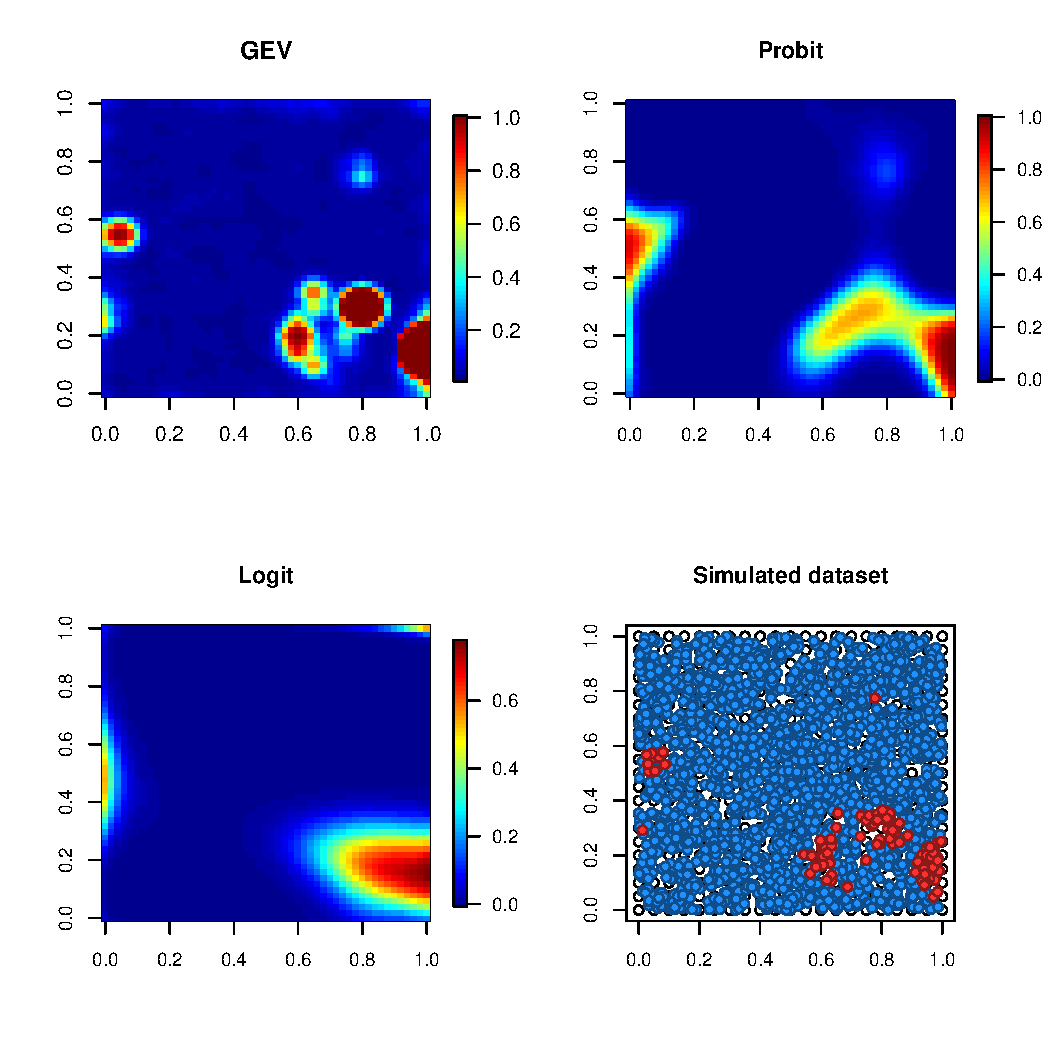
\includegraphics[width=\linewidth]{plots/post-med-2.pdf}
%   \caption{Posterior median $P(Y = 1)$ for spatial GEV, probit, and logistic regression for setting 2.}
%   \label{rbfig:post-med-2}
% \end{figure}

% \begin{figure}
%   % this figure comes from markdown/sim-hmc/predict-maps.R
%   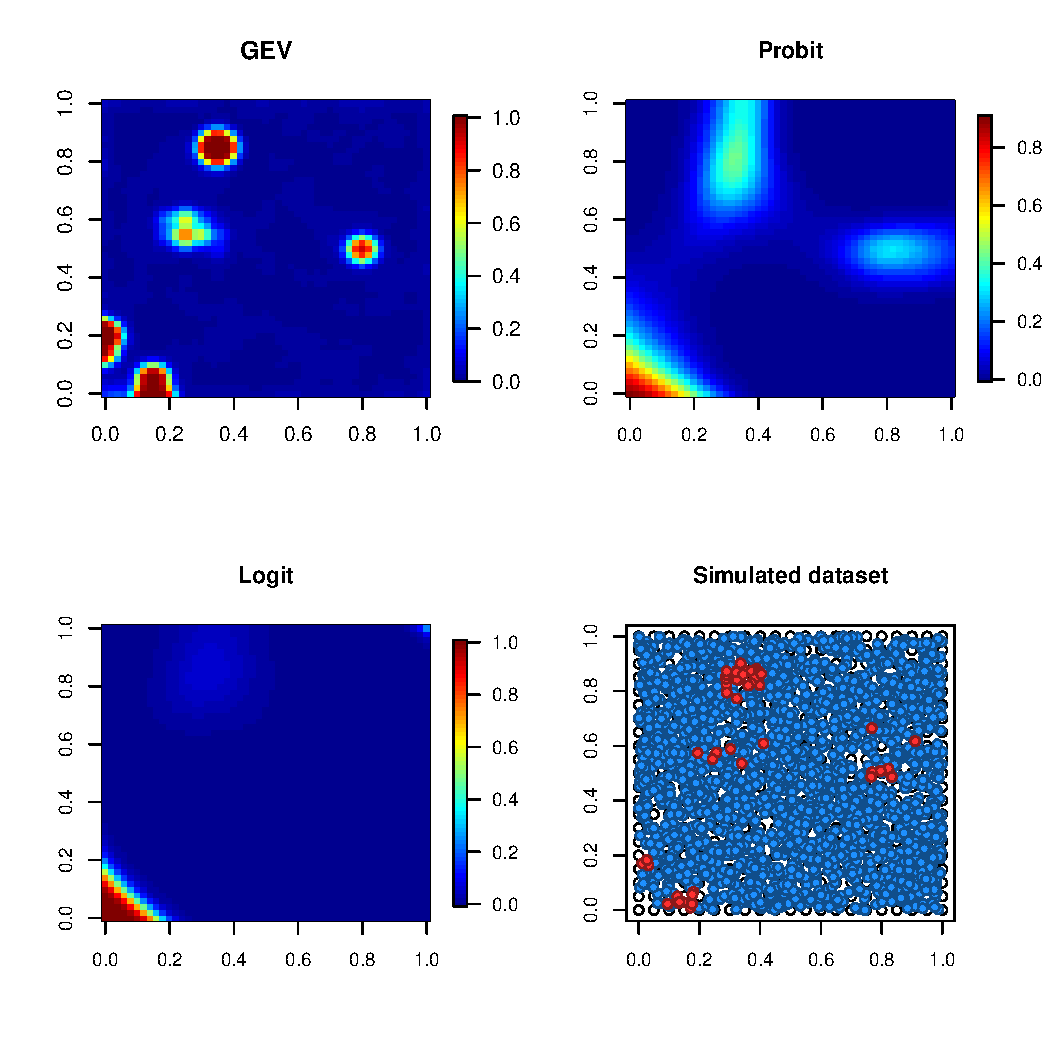
\includegraphics[width=\linewidth]{plots/post-med-3.pdf}
%   \caption{Posterior median $P(Y = 1)$ for spatial GEV, probit, and logistic regression for setting 3.}
%   \label{rbfig:post-med-3}
% \end{figure}

\section{Data analysis}\label{rbs:analysis}
\hl{Needs updating}

For the data analysis, we consider data from the eBirds dataset, a citizen-based observation network of bird sitings in the United States \citep{Sullivan2009}.
The data are publicly available from {\tt http://ebird.org}.
We use data from 2002, and focus on 10 different species.
\fref{rbfig:data2002} shows the sighting data for cattle egrets and vesper sparrows

\begin{figure}
  \centering
  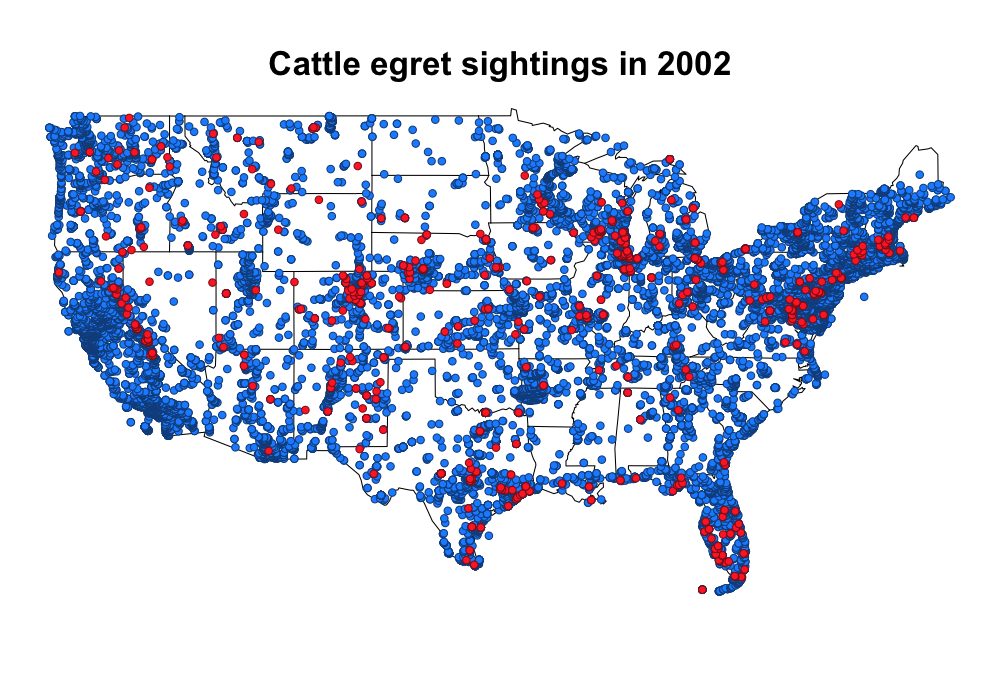
\includegraphics[width=0.47\linewidth]{plots/cattle_egret.png}
  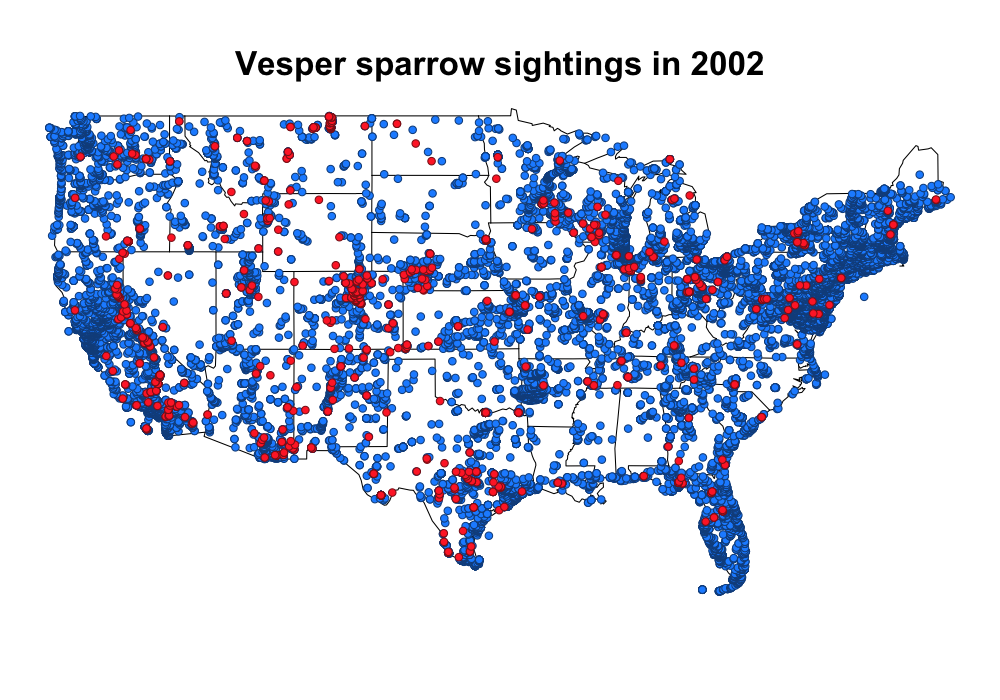
\includegraphics[width=0.47\linewidth]{plots/vesper_sparrow.png}
  \caption{Reported sighting for Cattle egret (left) and Vesper sparrow (right) in 2002}
  \label{rbfig:data2002}
\end{figure}

\section{Conclusions}\label{rbs:con}

\section*{Acknowledgments}

\appendix
\section{Appendices}
\subsection{Binary regression using the GEV link}\label{rba:rarebinary}
Here, we provide a brief review of the the GEV link of \citet{Wang2010}.
Let $Y_i \in \{0, 1\}, i = 1, \ldots, n$ be a collection of i.i.d. binary responses.
It is assumed that $Y_i = I(z_i > 0)$ where $I(\cdot)$ is an indicator function, $z_i = [1 - \xi \bX_i \bbeta]^{1 / \xi}$ is a latent variable following a GEV$(1, 1, 1)$ distribution, $\bX_i$ is the associated $p$-vector of covariates with first element equal to one for the intercept, and $\bbeta$ is a $p$-vector of regression coefficients.
Then, $Y_i \ind$ Bern$(\pi_i)$ where $\pi_i= 1 - \exp \left( -\frac{ 1 }{ z_i } \right)$.


\subsection{Derivation of the likelihood} \label{rba:likelihoodderivation}
We use the hierarchical max-stable spatial model given by \citet{Reich2012}. If at each margin, $Z_i \sim $ GEV$(1,1,1)$, then $Z_i | \theta_i \indep $ GEV$(\theta, \alpha \theta, \alpha)$. We reorder the data such that $Y_1=\ldots=Y_K=1$, and $Y_{K+1} = \ldots = Y_n = 0$. Then the joint likelihood conditional on the random effect $\theta$ is

\begin{align} \label{rbeq:joint_cond}
	P(Y_1=y_1,\ldots,Y_n=y_n) =& \prod_{ i \le K } \left\{ 1 - \exp \left[ - \left( \frac{ \theta_i }{ z_i } \right)^{ 1/\alpha} \right] \right \} \prod_{ i > K } \exp \left[ -\left( \frac{ \theta_i }{ z_i } \right)^{1/\alpha} \right] \nonumber \\[0.5em]
		=& \exp \left[ -\sum_{ i = K+1}^{ n }\left( \frac{ \theta_i }{ z_i } \right)^{1/\alpha} \right] - \exp \left[ -\sum_{ i = K+1}^{ n }\left( \frac{ \theta_i }{ z_i } \right)^{1/\alpha} \right] \sum_{ i = 1}^{K} \exp\left[ -\left( \frac{ \theta_i }{ z_i } \right)^{ 1/\alpha} \right] \nonumber\\
		&  + \exp \left[ -\sum_{ i = K+1}^{ n }\left( \frac{ \theta_i }{ z_i } \right)^{1/\alpha} \right] \sum_{ 1 < i < j \le K } \left\{ \exp \left[ - \left( \frac{ \theta_i }{ z_i } \right)^{ 1/\alpha} - \left( \frac{ \theta_j }{ z_j } \right)^{ 1/\alpha } \right] \right \} \nonumber \\[0.5em]
		& + \cdots + (-1)^K \exp\left[ - \sum_{ i = 1 }^{ n }\left( \frac{ \theta_i }{ z_i } \right)^{ 1/\alpha} \right]
\end{align}

Finally marginalizing over the random effect, we obtain

\begin{align} \label{rbeq:joint}
    P(Y_1=y_1,\ldots,Y_n=y_n) =&\int G(\bz | \bA) p( \bA | \alpha) d\bA. \nonumber\\[0.5em]
			=& \int \exp \left[ -\sum_{ i = K+1}^{ n }\left( \frac{ \theta_i }{ z_i } \right)^{1/\alpha} \right] - \exp \left[ -\sum_{ i = K+1}^{ n }\left( \frac{ \theta_i }{ z_i } \right)^{1/\alpha} \right] \sum_{ i = 1}^{K} \exp\left[ -\left( \frac{ \theta_i }{ z_i } \right)^{ 1/\alpha} \right] \nonumber\\
		&  + \exp \left[ -\sum_{ i = K+1}^{ n }\left( \frac{ \theta_i }{ z_i } \right)^{1/\alpha} \right] \sum_{ 1 < i < j \le K } \left\{ \exp \left[ - \left( \frac{ \theta_i }{ z_i } \right)^{ 1/\alpha} - \left( \frac{ \theta_j }{ z_j } \right)^{ 1/\alpha } \right] \right \} \nonumber \\[0.5em]
		& + \cdots + (-1)^K \exp\left[ - \sum_{ i = 1 }^{ n }\left( \frac{ \theta_i }{ z_i } \right)^{ 1/\alpha} \right] p( \bA | \alpha) d\bA.
\end{align}

Consider the first term in the summation,

\begin{align}
	\int \exp \left\{ -\sum_{ i = K+1}^{ n }\left( \frac{ \theta_i }{ z_i } \right)^{1/\alpha} \right\} p( \bA | \alpha) d\bA &= \int \exp \left\{ - \sum_{ i = K + 1 }^n \left( \frac{ \left[ \sum_{ l = 1 }^L  A_l w_{l}(\bs_i)^{1/\alpha} \right)^\alpha }{ z_i} \right]^{ 1/\alpha } \right \} p( \bA | \alpha) d\bA \nonumber \\[0.5em]
	 &= \int \exp \left\{ -\sum_{ i = K + 1}^n \sum_{ l = 1}^L A_l \left( \frac{ w_l (\bs_i) }{ z_i } \right)^{1/\alpha} \right \} p( \bA | \alpha) d\bA \nonumber \\[0.5em]
	 &=\exp\left\{-\sum_{ l = 1}^L \left[ \sum_{ i = K + 1 }^n \left( \frac{ w_l(\bs_i)}{ z_i} \right)^{1/\alpha} \right]^\alpha \right\}.
\end{align}

The remaining terms in equation \eref{rbeq:joint} are straightforward to obtain, and after integrating out the random effect, the joint density for $K = 0, 1, 2$ is given by
\begin{align}\label{rbeq:pmf}
  P(Y_1=y_1,\ldots,Y_n=y_n) =  \left\{
    \begin{array}{ll}
      G(\bz) & K=0 \\
      G(\bz_{(1)})-G(\bz) & K=1 \\
      G(\bz_{(12)})-G(\bz_{(1)})-G(\bz_{(2)})+G(\bz) & K=2
    \end{array}
  \right.
\end{align}
where
\begin{align*}
  G[\bz_{(1)}] &= P[Z(\bs_2)<z(\bs_2),\ldots,Z(\bs_n)<z(\bs_n)] \\
  G[\bz_{(2)}] &= P[Z(\bs_1)<z(\bs_1),Z(\bs_3)<z(\bs_3),\ldots,Z(\bs_n)<z(\bs_n)]\\
  G[\bz_{(12)}] &= P[Z(\bs_3)<z(\bs_3),\ldots,Z(\bs_n)<z(\bs_n)].
\end{align*}
Similar expressions can be derived for all $K$, but become cumbersome for large $K$.

% \subsection{Proof that $\lim_{\beta \rightarrow \infty} \kappa(\beta) = \chi$} \label{rba:chi}
% Assume that $Z_1$ and $Z_2$ are both GEV$(\beta, 1, 1)$ so that the probability of $Y_i$ decreases to zero as $\beta$ increases.
% Recall from \sref{rbs:spatdep} that
% \begin{align*}
%   P_A(\beta) &= 1 - 2 \exp\left\{ -\frac{1}{\beta} \right\} + 2 \exp\left\{-\frac{\vartheta(\bs_1, \bs_2)}{\beta}  \right\} \\
%   P_E(\beta) &= 1 - 2 \exp \left\{ -\frac{1}{\beta} \right\} + 2 \exp \left\{ -\frac{2}{\beta} \right\}.
% \end{align*}
% Then
% \begin{align} \label{rbeq:kappabeta}
%   \kappa(\beta) &= \frac{P_A(\beta) - P_E(\beta)}{1 - P_E(\beta)} = \frac{\exp\left\{-\frac{\vartheta(\bs_1, \bs_2) - 1}{\beta}  \right\} - \exp \left\{ -\frac{1}{\beta} \right\}}{1 - \exp \left\{ -\frac{1}{\beta} \right\}}.
% \end{align}
% where $\vartheta(\bs_1, \bs_2)$ is defined as in \sref{rbs:spatdep}.
% So,
% \begin{align}
%   \kappa =
% \end{align}

\subsection{Simulation study pairwise difference results} \label{rba:pdiffs}
\hl{Needs updating}

The following tables show the methods that have significantly different Brier scores when using a Wilcoxon-Nemenyi-McDonald-Thompson test.
In each column, different letters signify that the methods have significantly different Brier scores.

\begin{table}[htbp]
  \centering
  \caption{Pairwise BS comparisons}
  \label{rbtbl:pwbssim}
  \begin{tabular}{|l|cc|cc|c|ccc|cc|cc|}
  \cline{2-13}
  \multicolumn{1}{c}{} & \multicolumn{2}{|c}{Setting 1} & \multicolumn{2}{|c}{Setting 2} & \multicolumn{1}{|c}{Setting 3} & \multicolumn{3}{|c}{Setting 4} & \multicolumn{2}{|c}{Setting 5} & \multicolumn{2}{|c|}{Setting 6}\\
  \hline
  Method 1 & A &   & A &   & A &   &   & C &   & B &   & B \\
  \hline
  Method 2 & A & B &   & B & A &   & B &   & A &   & A &   \\
  \hline
  Method 3 &   & B &   & B & A & A &   &   & A & B & A &   \\
  \hline
  \end{tabular}
\end{table}

% \begin{table}[htbp]
%   \centering
%   \caption{Pairwise AUC comparisons}
%   \label{rbtbl:pwaucsim}
%   \begin{tabular}{|l|cc|}
%   \multicolumn{1}{c}{} & \multicolumn{2}{|c}{Setting 1} \\
%   \hline
%   Method 1 & A &   & A &   \\
%   \hline
%   Method 2 & A & B & A & B \\
%   \hline
%   Method 3 &   & B &   & B \\
%   \hline
%   \end{tabular}
% \end{table}


\begin{singlespace}
\bibliographystyle{rss}
\bibliography{library}
\end{singlespace}


\end{document}

